\documentclass[tikz,border=8pt]{standalone}
\usepackage{amsmath,amssymb}
\usetikzlibrary{arrows.meta,automata,positioning,quotes}
\begin{document}
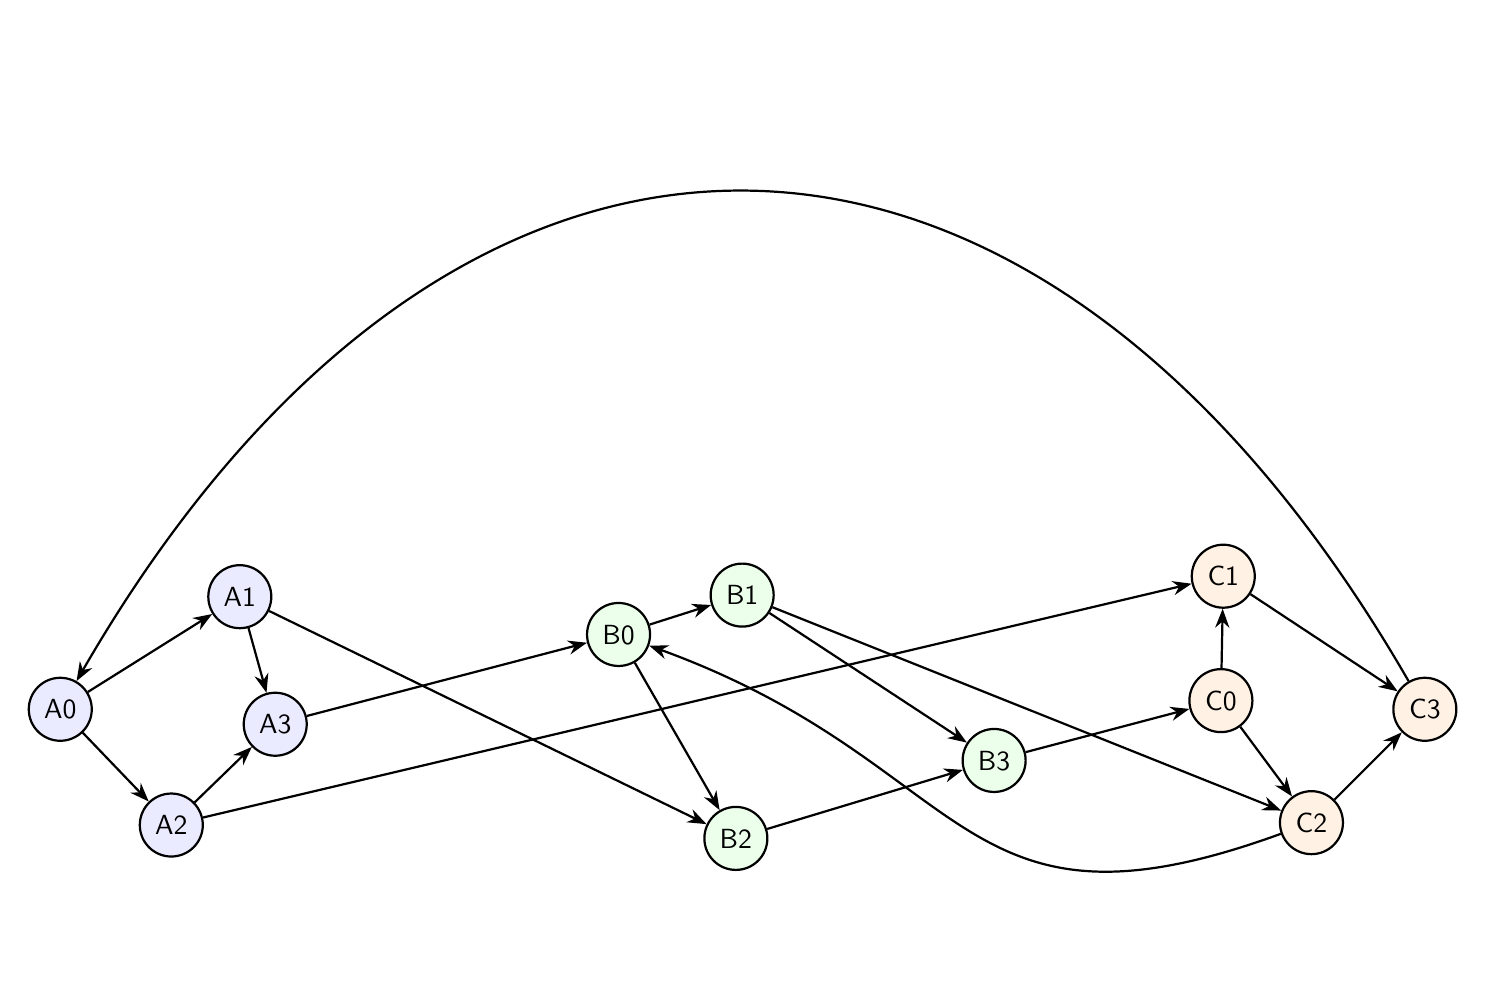
\begin{tikzpicture}[x=1cm,y=1cm]
\tikzset{
  graphnode/.style={circle,draw,thick,minimum size=8mm,inner sep=1pt,font=\sffamily},
  directed/.style={-{Stealth[length=2.4mm]},thick},
  undirected/.style={thick}
}
\node[graphnode,fill=blue!8] (n_A0) at (-2.70,-0.01) {A0};
\node[graphnode,fill=blue!8] (n_A1) at (-0.42,1.42) {A1};
\node[graphnode,fill=blue!8] (n_A2) at (-1.29,-1.48) {A2};
\node[graphnode,fill=blue!8] (n_A3) at (0.03,-0.20) {A3};
\node[graphnode,fill=green!8] (n_B0) at (4.39,0.94) {B0};
\node[graphnode,fill=green!8] (n_B1) at (5.96,1.44) {B1};
\node[graphnode,fill=green!8] (n_B2) at (5.88,-1.65) {B2};
\node[graphnode,fill=green!8] (n_B3) at (9.16,-0.66) {B3};
\node[graphnode,fill=orange!10] (n_C0) at (12.04,0.10) {C0};
\node[graphnode,fill=orange!10] (n_C1) at (12.07,1.68) {C1};
\node[graphnode,fill=orange!10] (n_C2) at (13.19,-1.45) {C2};
\node[graphnode,fill=orange!10] (n_C3) at (14.63,-0.01) {C3};
\draw[directed] (n_A0) -- (n_A1);
\draw[directed] (n_A0) -- (n_A2);
\draw[directed] (n_A1) -- (n_A3);
\draw[directed] (n_A2) -- (n_A3);
\draw[directed] (n_B0) -- (n_B1);
\draw[directed] (n_B0) -- (n_B2);
\draw[directed] (n_B1) -- (n_B3);
\draw[directed] (n_B2) -- (n_B3);
\draw[directed] (n_C0) -- (n_C1);
\draw[directed] (n_C0) -- (n_C2);
\draw[directed] (n_C1) -- (n_C3);
\draw[directed] (n_C2) -- (n_C3);
\draw[directed] (n_A3) -- (n_B0);
\draw[directed] (n_B3) -- (n_C0);
\draw[directed] (n_A1) -- (n_B2);
\draw[directed] (n_A2) -- (n_C1);
\draw[directed] (n_B1) -- (n_C2);
\draw[directed] (n_C3) to[out=120,in=60,looseness=1.45,dashed] (n_A0);
\draw[directed] (n_C2) to[out=-160,in=-20,looseness=1.35,dashed] (n_B0);
\end{tikzpicture}
\end{document}
